\prefacesection{Abstract}
Having now become a mass cultural phenomenon, video games are a unique medium, in fact they are very different from other types of media while incorporating their various languages. It has been authoritatively affirmed that, it is interactivity that has distinguished video games from other forms of mass media entertainment; precisely this characteristic allows the video game to exercise a potential of immersion and attraction that other media do not have.

With hundreds of millions of people playing interactive games regularly today, gaming is fast becoming a dominant player in the entertainment industry.	It is certainly a continuously growing sector that has never undergone stoppages over the years.

\begin{figure}[H]
	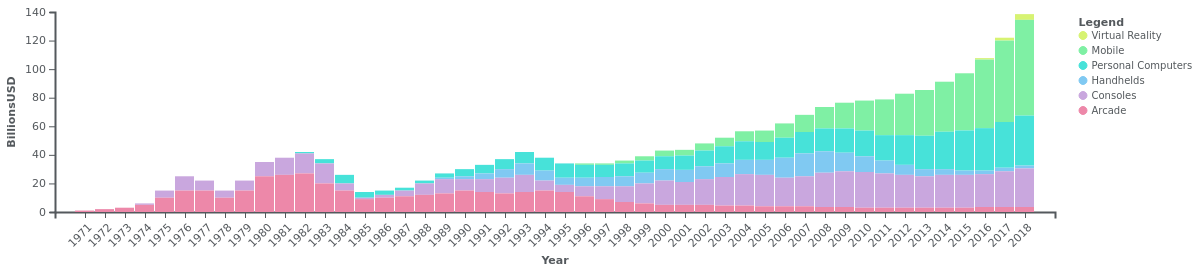
\includegraphics[width=\linewidth]{immagini/valore_commerciale_giochi_globale.png}
	\caption{Value of global video game market in USD billion. Source: wikipedia.org}
	\label{fig:valore_commerciale_giochi_globale}
\end{figure}

As the speed of network connections continues to increase, we are moving towards a new digital age as part of a communications revolution that will affect every aspect of consumers' lives, not least the change it brings in terms of options in the entertainment industry. The challenge is to invent content consumption patterns of existing and new types of content and services. One of these opportunities is realized through two technologies that have now become part of everyday life: streaming and cloud computing.

This project involves the creation of a cloud gaming platform, which allows the direct and on-demand audio-video streaming of video games, from a remote server, to a web browser (computer, console, telephone, TV). The game is archived, played, and rendered on a remote server; the input (keyboard, gamepad) is sent from the web browser to the server.

In this way, games can be accessed regardless of the operating system and hardware capabilities of the client used, the only prerequisite is a 1.5 Mbps network connection. In addition, the system allows the user to start playing immediately. Finally, the platform indirectly guarantees the management of digital rights (DRM\footnote{Digital rights management, a set of access control technologies for restricting the use of proprietary hardware and copyrighted works.}) for publishers.

The system is based on the MAME\footnote{Multiple Arcade Machine Emulator, is an emulator designed to recreate the hardware of arcade game systems in software on modern personal computers, released under the GNU-GPL license.} emulator that can run on Linux, Windows and macOS, supports couch multiplayer up to 4 players and a library of over 7,000 games.

Since no configuration is required and the user interface is made up of web pages, it makes the system easily usable by all groups of users which will be encouraged to play the games that made the history of video games.